% !TEX program = xelatex
\documentclass[11pt, a4paper]{article}

\usepackage{fontspec}
\usepackage{xetexko}
\usepackage[margin=2.5cm, top=3cm, bottom=3cm]{geometry}
\usepackage{graphicx}
\usepackage{booktabs}
\usepackage{tabularx}
\usepackage{xcolor}
\usepackage{hyperref}
\usepackage{titlesec}
\usepackage{fancyhdr}
\usepackage{enumitem}
\usepackage{float}
\usepackage{caption}
\usepackage{array}
\usepackage{colortbl}
\usepackage{tikz}

\setmainfont{Apple SD Gothic Neo}
\setsansfont{Apple SD Gothic Neo}
\setmonofont{Menlo}

\definecolor{darkblue}{HTML}{1A5276}
\definecolor{medblue}{HTML}{2980B9}
\definecolor{lightblue}{HTML}{D4E6F1}
\definecolor{darkgray}{HTML}{2C3E50}
\definecolor{lightgray}{HTML}{F2F3F4}
\definecolor{green}{HTML}{27AE60}

\hypersetup{colorlinks=true, linkcolor=darkblue, urlcolor=medblue}

\titleformat{\section}
  {\Large\bfseries\color{darkblue}}{\thesection.}{0.5em}{}
  [\vspace{-0.5em}\textcolor{medblue}{\rule{\textwidth}{0.5pt}}]
\titleformat{\subsection}
  {\large\bfseries\color{darkblue}}{\thesubsection}{0.5em}{}

\pagestyle{fancy}
\fancyhf{}
\fancyhead[L]{\small\color{darkgray}매장별 주간 매출 예측}
\fancyhead[R]{\small\color{darkgray}BDM Lab}
\fancyfoot[C]{\small\color{darkgray}\thepage}
\renewcommand{\headrulewidth}{0.4pt}

\newcolumntype{L}[1]{>{\raggedright\arraybackslash}p{#1}}
\newcolumntype{C}[1]{>{\centering\arraybackslash}p{#1}}

\begin{document}

% ── COVER ─────────────────────────────────────────────
\thispagestyle{empty}
\begin{center}
\vspace*{3.5cm}

{\fontsize{30}{36}\selectfont\bfseries\color{darkblue}
각 매장이 다음 주에\\[10pt]
얼마를 팔지, AI가 맞춘다.}

\vspace{1.5cm}

{\Large\color{darkgray}
284개 슈퍼마켓 매장 · 52주 데이터 · 주간 매출 예측}

\vspace{0.8cm}
\textcolor{medblue}{\rule{8cm}{0.8pt}}
\vspace{2cm}

\begin{tikzpicture}
\node[fill=lightblue, rounded corners=8pt, minimum width=14cm, minimum height=3.5cm] {
  \begin{minipage}{13cm}
  \centering
  \vspace{4pt}
  {\large\bfseries\color{darkblue} 예측 성능}\\[12pt]
  \begin{minipage}[t]{0.3\textwidth}\centering
    {\fontsize{36}{40}\selectfont\bfseries\color{darkblue}284개}\\[4pt]
    {\normalsize\color{darkgray}매장 매출 예측}
  \end{minipage}\hfill
  \begin{minipage}[t]{0.3\textwidth}\centering
    {\fontsize{36}{40}\selectfont\bfseries\color{green}82\%}\\[4pt]
    {\normalsize\color{darkgray}예측 설명력}
  \end{minipage}\hfill
  \begin{minipage}[t]{0.3\textwidth}\centering
    {\fontsize{36}{40}\selectfont\bfseries\color{darkblue}2만건}\\[4pt]
    {\normalsize\color{darkgray}검증 완료}
  \end{minipage}
  \vspace{4pt}
  \end{minipage}
};
\end{tikzpicture}

\vspace{3cm}

{\large\color{darkgray}
빅데이터마케팅 랩 · 한양대학교 임보람 교수\\[8pt]
2026년 4월}

\end{center}

\newpage

% ═══════════════════════════════════════════════════════
\section{무엇을 예측하는가}

슈퍼마켓 284개 매장 각각의 \textbf{다음 주 매출}을 예측합니다.

\begin{itemize}[itemsep=6pt]
  \item \textbf{매장 매출:} 각 매장이 다음 주에 얼마를 팔지
  \item \textbf{고객 구매 패턴:} 고객이 몇 명 올지, 장바구니에 무엇을 담을지
  \item \textbf{채널별 분리:} 온라인 주문과 오프라인 매장을 각각 따로 예측
\end{itemize}

52주간의 실제 거래 데이터로 학습하고, \textbf{14주간의 미래 데이터}로 검증했습니다. 학습에 쓰지 않은 데이터로만 평가했기 때문에 실전 성능과 동일합니다.

\begin{table}[H]
\centering
\large
\begin{tabular}{L{6cm} C{3.5cm} C{3.5cm}}
\toprule
\rowcolor{lightblue} & \textbf{온라인 주문} & \textbf{오프라인 매장} \\
\midrule
\textbf{예측 설명력 (R²)} & \textcolor{darkblue}{\textbf{0.82}} & 0.66 \\[4pt]
매장 수 & 225개 & 281개 \\[4pt]
검증 건수 & 9,878건 & 11,929건 \\
\bottomrule
\end{tabular}
\end{table}

\begin{figure}[H]
\centering
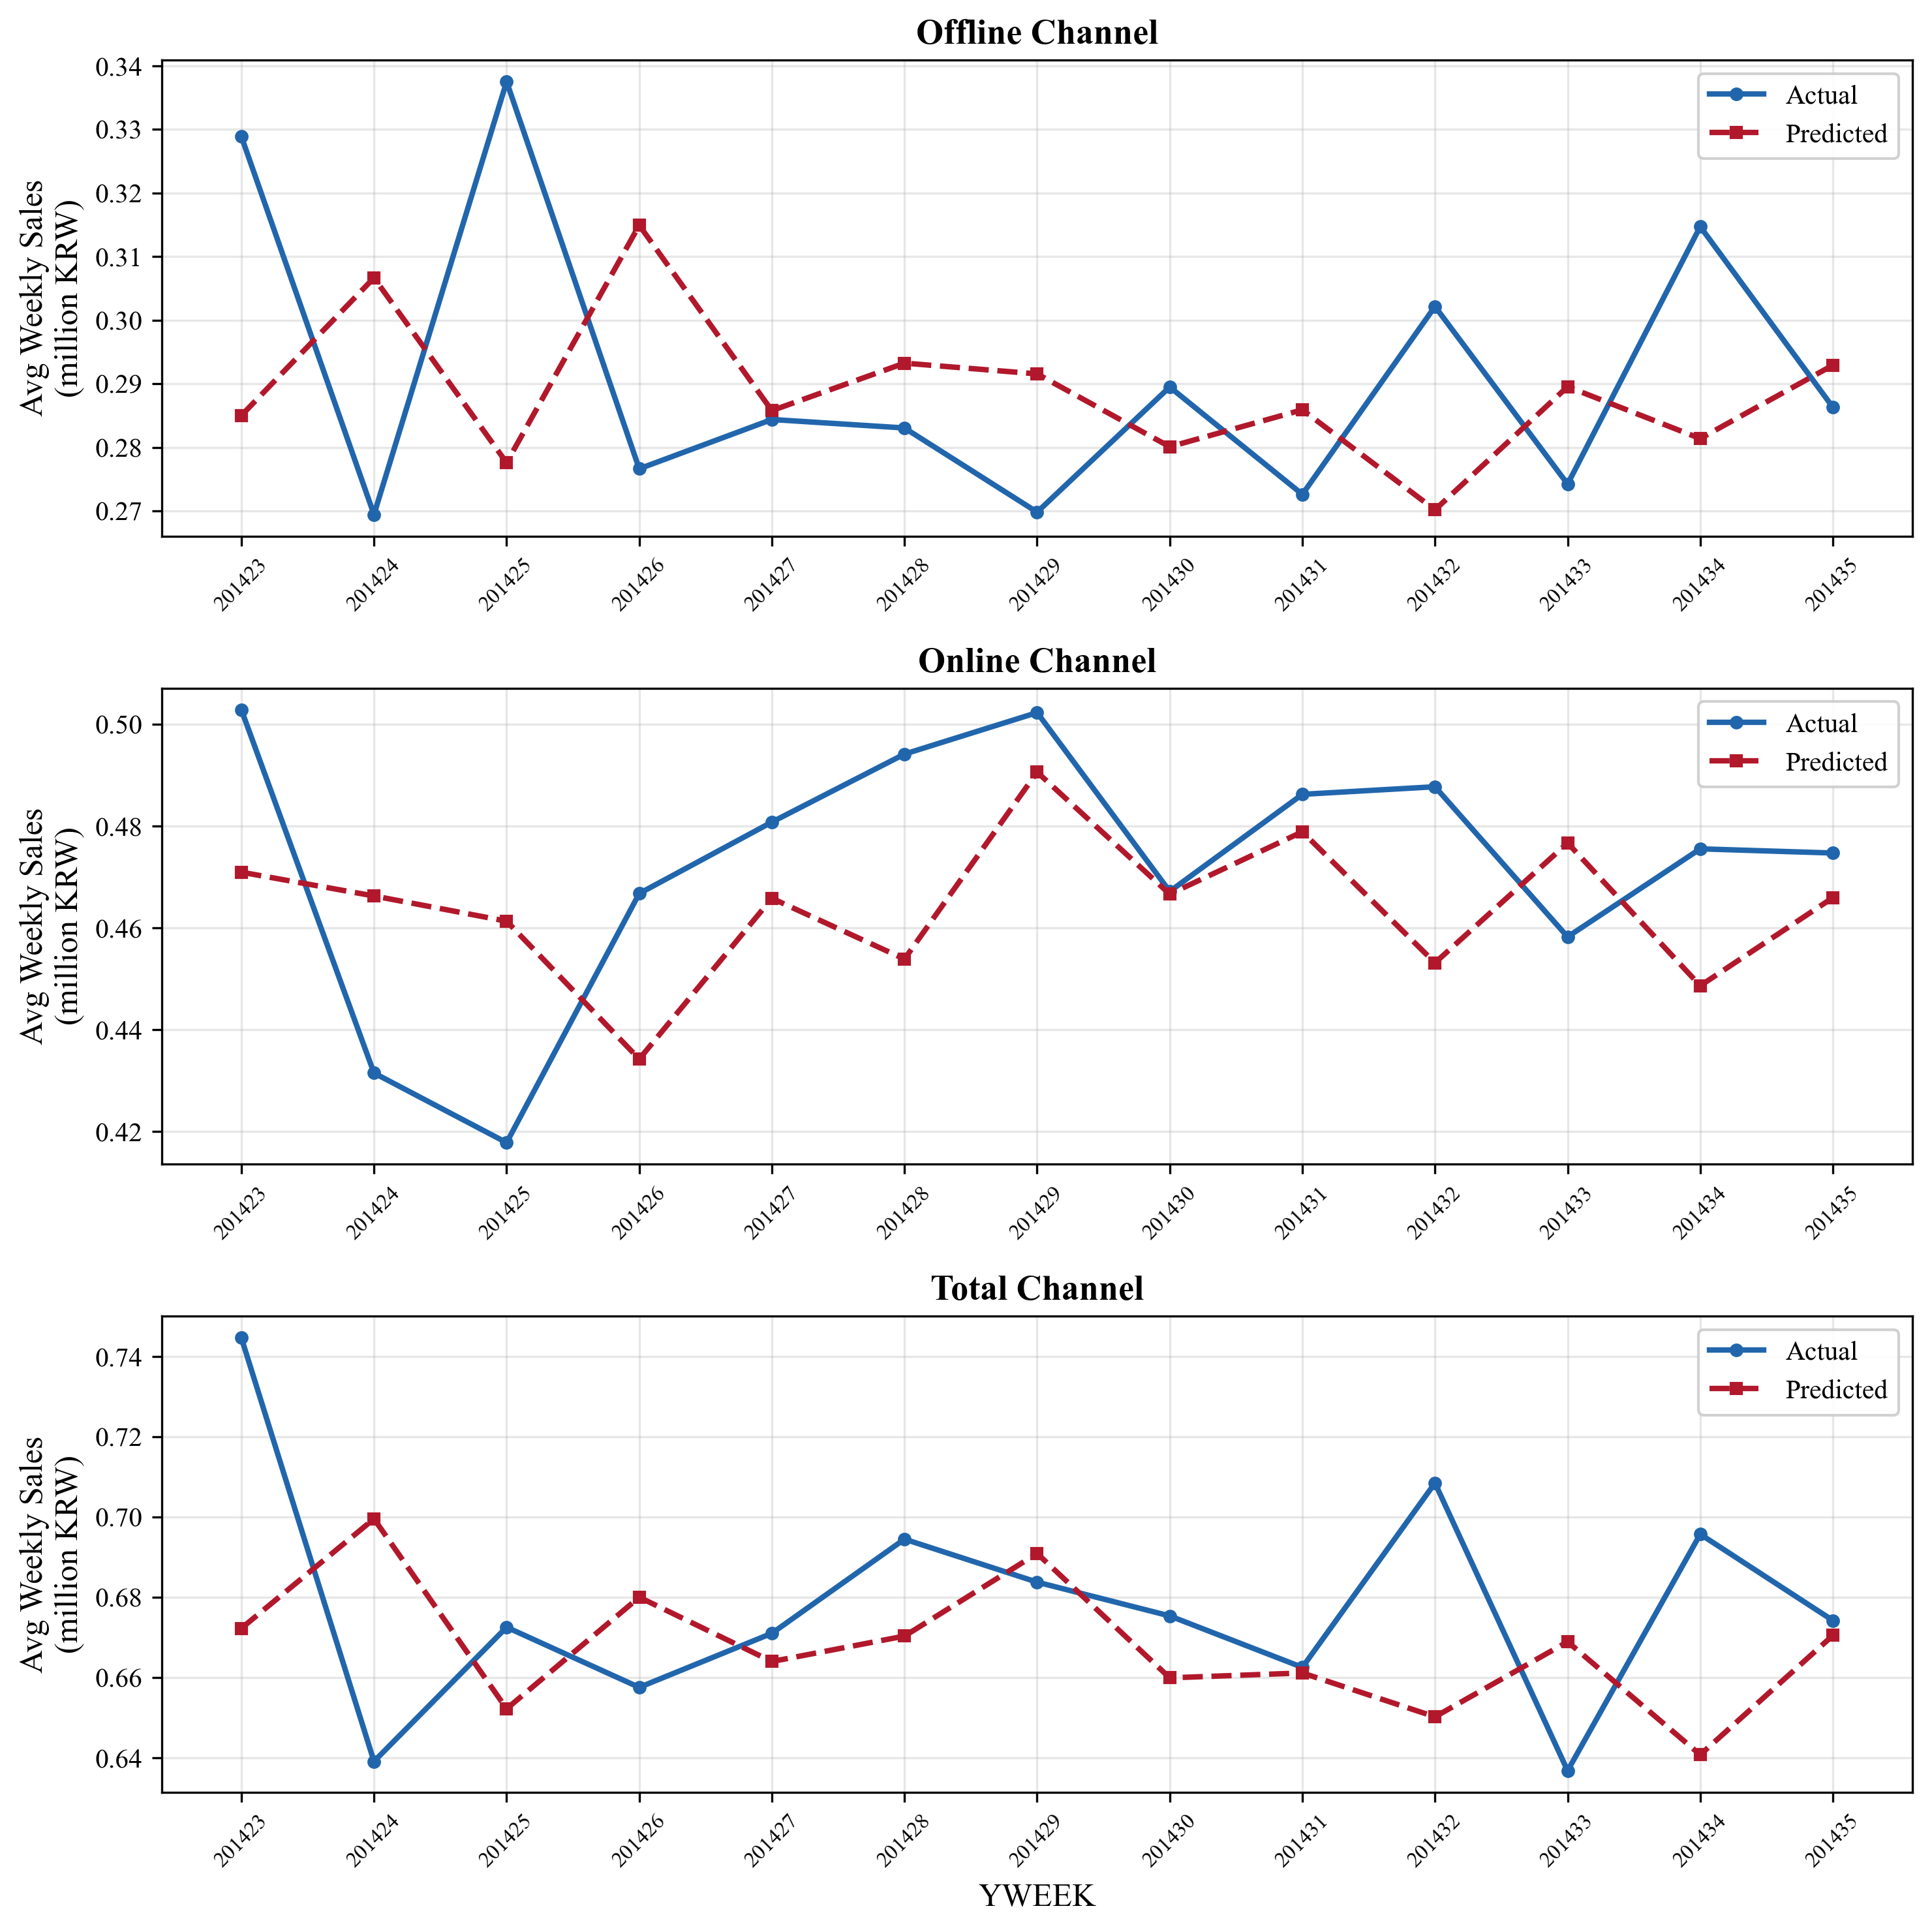
\includegraphics[width=0.85\textwidth]{figure4_actual_vs_predicted.png}
\caption{14주간 실제 매출(실선) vs AI 예측(점선) — 거의 겹친다}
\end{figure}

\newpage

% ═══════════════════════════════════════════════════════
\section{매출을 결정하는 핵심 요인}

353개 변수를 동시에 분석했습니다. 매장 주변 인구, 경쟁 매장, 프로모션, 고객 행동 등. 이 중 \textbf{매출을 압도적으로 결정하는 것은 고객의 구매 패턴}이었습니다.

\begin{table}[H]
\centering
\begin{tabularx}{\textwidth}{C{1cm} L{4.5cm} X}
\toprule
\rowcolor{lightblue} & \textbf{예측 요인} & \textbf{설명} \\
\midrule
\textbf{1} & 고객이 몇 명 오는가 & 방문 고객 수가 매출의 가장 강력한 예측 변수. 다른 모든 변수를 압도. \\[6pt]
\textbf{2} & 장바구니에 무엇을 담는가 & 어떤 카테고리 상품을 사는지, 몇 가지를 사는지. \\[6pt]
\textbf{3} & 지난주에 얼마를 팔았는가 & 직전 주 매출은 관성 효과로 다음 주를 예측하는 좋은 기준선. \\[6pt]
\textbf{4} & 장바구니 크기 & 한 번에 몇 개를 사는지, 1인당 구매 금액. \\
\bottomrule
\end{tabularx}
\caption{매출 예측 변수 중요도 순위}
\end{table}

\subsection{반대로, 효과가 거의 없었던 것}

\begin{itemize}[itemsep=4pt]
  \item \textbf{프로모션/할인} → 고객 구매 이력이 이미 반영하고 있음
  \item \textbf{주변 경쟁 매장 수} → 추가 예측력 거의 없음
  \item \textbf{지역 인구통계} → 마찬가지로 추가 효과 미미
\end{itemize}

\colorbox{lightblue}{%
\begin{minipage}{0.95\textwidth}\vspace{8pt}
\textbf{결론:} 상권 분석에 돈을 쓰기 전에, \textbf{자사 고객 데이터를 먼저 분석}하는 것이 매출 예측에 훨씬 더 효과적입니다.
\vspace{8pt}
\end{minipage}%
}

\begin{figure}[H]
\centering
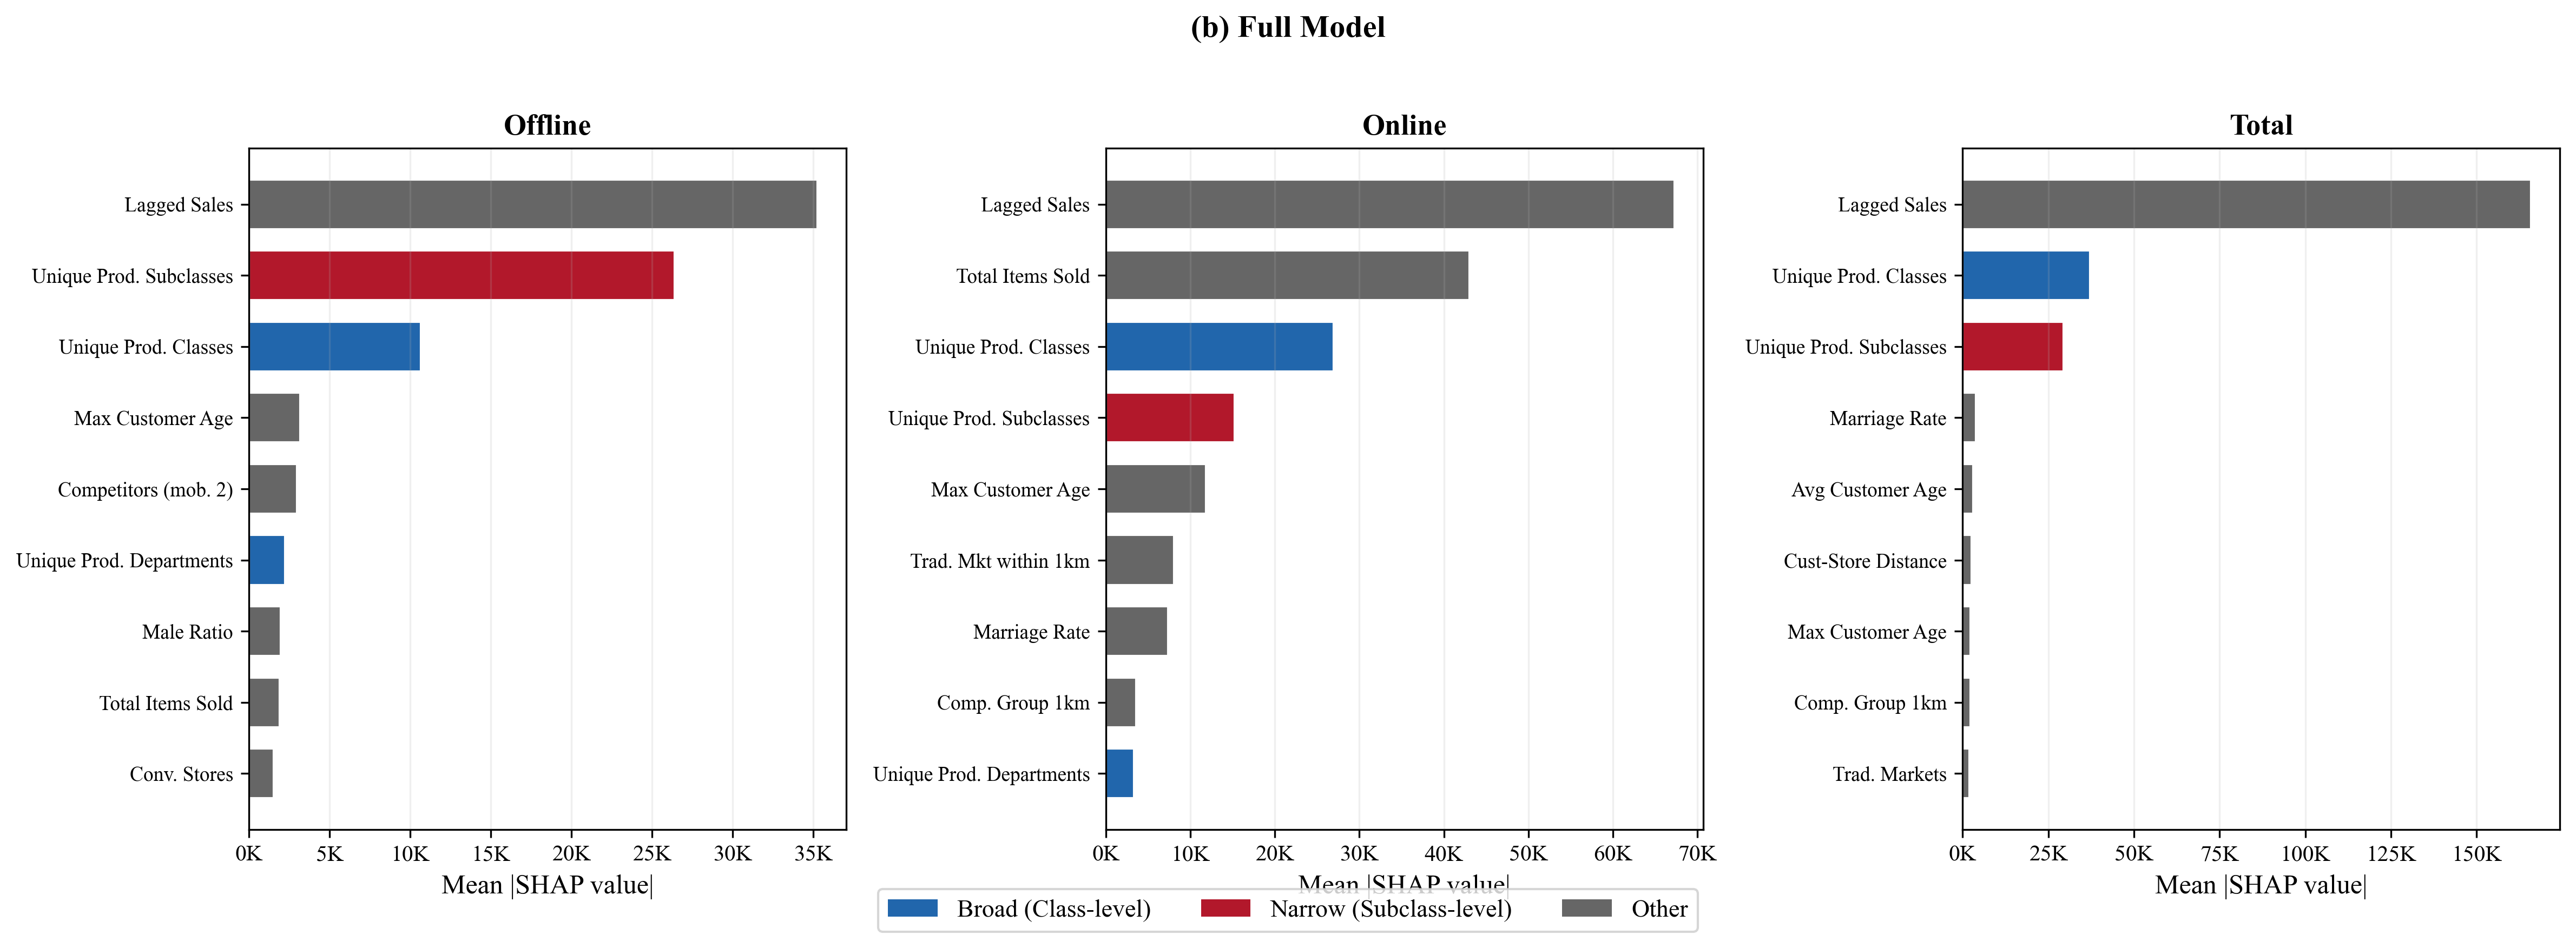
\includegraphics[width=0.9\textwidth]{figure5b_shap_full.png}
\caption{AI가 매출을 예측할 때 가장 많이 참고하는 정보 (SHAP 분석)}
\end{figure}

\newpage

% ═══════════════════════════════════════════════════════
\section{핵심 발견: 온라인과 오프라인 고객은 다른 단위로 사고한다}

AI 모델이 매출을 예측할 때, 상품 정보를 어느 수준에서 보느냐가 채널별로 완전히 달랐습니다.

\begin{table}[H]
\centering
\large
\begin{tabular}{L{4cm} C{4cm} C{4cm}}
\toprule
\rowcolor{lightblue} & \textbf{온라인 고객} & \textbf{오프라인 고객} \\
\midrule
\textbf{의사결정 단위} & 큰 카테고리 (Class) & 세부 카테고리 (Subclass) \\[6pt]
\textbf{예시} & ``유제품을 샀는가'' & ``크림치즈를 골랐는가'' \\[6pt]
\textbf{쇼핑 방식} & 검색 → 필터 → 장바구니 & 보고 → 만지고 → 고르기 \\[6pt]
\textbf{SHAP 중요도} & \textcolor{darkblue}{\textbf{26,976}} vs 15,276 & 10,664 vs \textbf{26,421} \\[4pt]
\textbf{우위} & \textcolor{darkblue}{\textbf{큰 카테고리 1.8배}} & \textbf{세부 카테고리 2.5배} \\
\bottomrule
\end{tabular}
\caption{채널별 상품 분류 수준의 중요도 비교 (4/4 모델 100\% 일관)}
\end{table}

\colorbox{lightblue}{%
\begin{minipage}{0.95\textwidth}\vspace{8pt}
\textbf{실무 원칙:}
\begin{itemize}[itemsep=3pt, leftmargin=1.5em]
  \item \textbf{온라인:} 카테고리 단위로 구색을 기획하라. ``유제품 10종''이 중요하지, ``어떤 크림치즈''는 덜 중요하다.
  \item \textbf{오프라인:} 세부 상품 단위로 진열을 큐레이션하라. ``어떤 크림치즈를 눈높이에 놓는가''가 매출을 바꾼다.
\end{itemize}
\vspace{4pt}
\end{minipage}%
}

\begin{figure}[H]
\centering
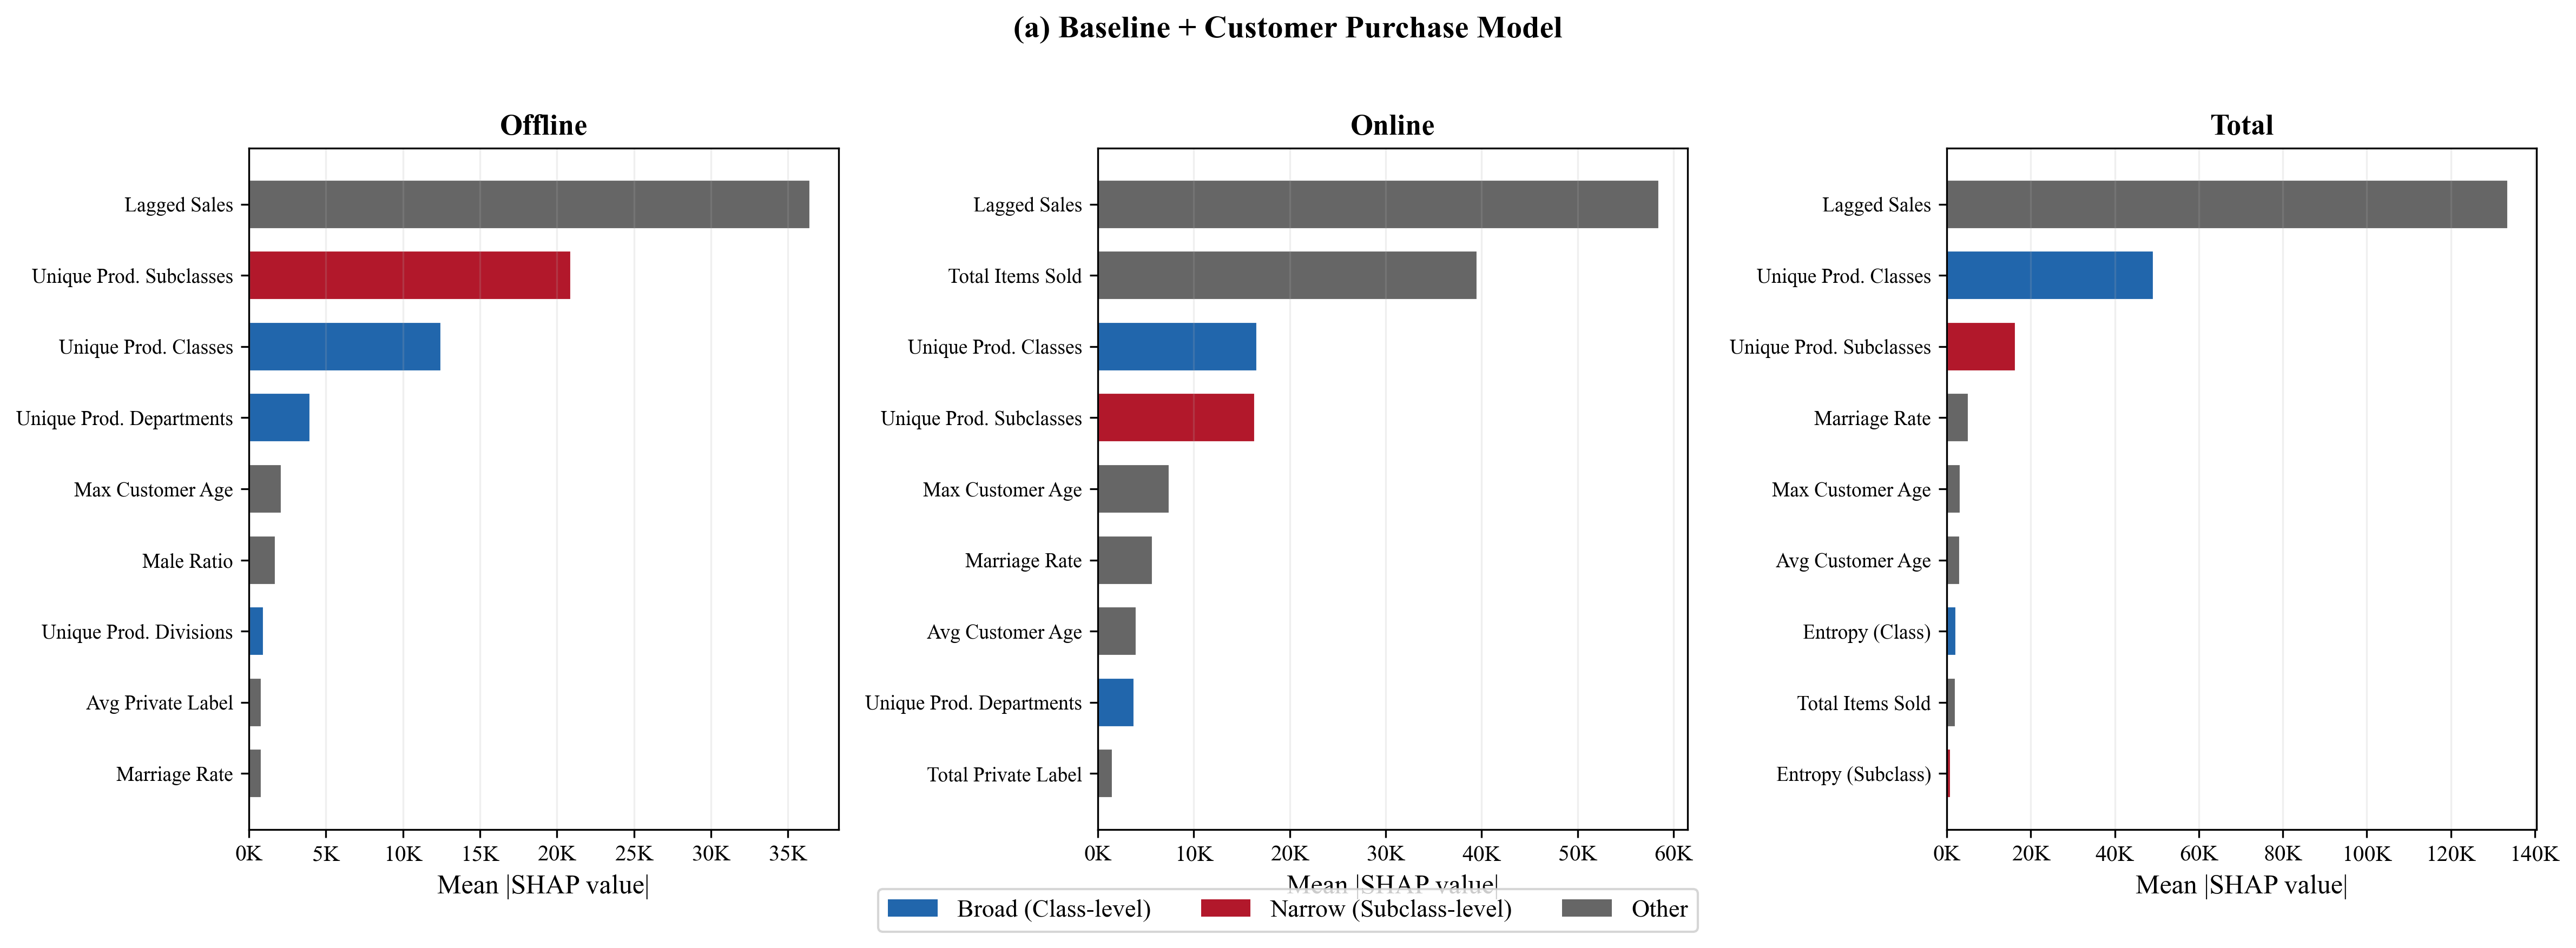
\includegraphics[width=0.9\textwidth]{figure5a_shap_custpurchase.png}
\caption{온라인에서는 큰 카테고리(파랑)가, 오프라인에서는 세부 카테고리(빨강)가 상위}
\end{figure}

\newpage

% ═══════════════════════════════════════════════════════
\section{왜 예측이 되는가 — 고객은 습관적으로 산다}

500명의 고객을 추적해서 확인했습니다.

\begin{table}[H]
\centering
\large
\begin{tabular}{L{6cm} C{4cm} C{4cm}}
\toprule
\rowcolor{lightblue} & \textbf{온라인 고객} & \textbf{오프라인 고객} \\
\midrule
장바구니 반복률 & \textcolor{darkblue}{\textbf{높음 (+26.3\%)}} & 기준 \\[4pt]
수요 변동성 & 낮음 ($-$2.3\%) & 기준 \\
\bottomrule
\end{tabular}
\end{table}

고객은 생각보다 습관적으로 삽니다. 매주 비슷한 물건을, 비슷한 금액만큼. 이 \textbf{``구매 관성''}이 AI가 매출을 맞출 수 있는 근본적인 이유입니다.

특히 온라인 주문은 검색$\rightarrow$장바구니$\rightarrow$결제의 목적형 구매라서 반복률이 더 높고, 따라서 예측 정확도도 높습니다.

% ═══════════════════════════════════════════════════════
\section{적용 가능 영역}

\begin{table}[H]
\centering
\begin{tabularx}{\textwidth}{C{0.8cm} L{4cm} X}
\toprule
\rowcolor{lightblue} & \textbf{적용 영역} & \textbf{기대 효과} \\
\midrule
\textbf{1} & 재고 최적화 & 매장별 다음 주 판매량을 알면, 과잉 재고와 품절을 동시에 줄인다 \\[6pt]
\textbf{2} & 인력 배치 & 매출이 높을 것으로 예측된 매장에 인력을 더 배치 \\[6pt]
\textbf{3} & 신규 매장 매출 추정 & 유사 고객 프로필의 기존 매장 데이터로 사전 추정 \\[6pt]
\textbf{4} & 고객 이탈 감지 & 구매 패턴이 변하는 고객을 조기 발견 \\[6pt]
\textbf{5} & 채널 전략 & 온라인과 오프라인의 다른 구매 패턴에 맞춘 별도 전략 수립 \\
\bottomrule
\end{tabularx}
\caption{적용 가능 영역}
\end{table}

\vspace{1cm}

\begin{center}
\textcolor{medblue}{\rule{6cm}{0.5pt}}\\[12pt]
{\large\color{darkgray}
빅데이터마케팅 랩\\[4pt]
한양대학교 경영대학 임보람 교수\\[4pt]
brlim@hanyang.ac.kr\\[4pt]
bigdatamarketinglab.com}
\end{center}

\vspace{0.5cm}
{\footnotesize\color{darkgray} 이 연구의 학술 버전은 Journal of Retailing and Consumer Services에 게재 확정되었습니다.}

\end{document}
